\documentclass{beamer}

\usepackage{graphicx}
\usepackage{mathtools}

\begin{document}
    \title{Demystifying Haskell}
    \subtitle{An in-depth examination of the Fibonacci sequence.}
    \author{Andrew Rademacher}


    \frame{\titlepage}

    \begin{frame}
        \frametitle{The Fibonacci Sequence}

        \begin{columns}[c]
            \begin{column}[T]{5cm}
                \begin{itemize}
                    \item Sequence is infinite
                    \item Sequence is self-referencing
                    \item Values grow exponentially
                    \item Values are always positive
                \end{itemize}
            \end{column}
            \begin{column}[T]{5cm}
                \begin{figure}
                    \centering
                    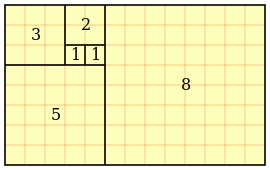
\includegraphics[height=3cm]{./fibs/images/FibonacciBlocks.png}
                \end{figure}

                \begin{figure}
                    \centering
                    \begin{math}
                        \left\{1,1,2,3,5,8...\right\}
                    \end{math}
                \end{figure}
               
                \begin{figure}
                    \centering
                    \begin{math}
                        F_{n} = F_{n-1} + F_{n-2}
                    \end{math}
                \end{figure}
            \end{column}
        \end{columns}
    \end{frame}
\end{document}
